\mode*

\section{Moduler}

\begin{frame}[fragile]
  \mintinline[fontsize=\huge]{python}|import module|
\end{frame}

\subsection{Hur?}

\begin{frame}[fragile]
  \begin{example}[good\textunderscore{}module.py]
    \inputminted[firstline=3,highlightlines=7]{python}{examples/good_module.py}
  \end{example}

  \begin{example}[bad\textunderscore{}module.py]
    \inputminted[firstline=3]{python}{examples/bad_module.py}
  \end{example}
\end{frame}


\subsection{Varför?}

%\begin{frame}[fragile]
%  \begin{example}[input\textunderscore{}type.py, del 1]
%    \inputminted[firstline=14]{python}{examples/input_type.py}
%  \end{example}
%\end{frame}

\begin{frame}[fragile]
  \begin{example}[input\textunderscore{}type.py]
    \inputminted[firstline=1,lastline=13]{python}{examples/input_type.py}
  \end{example}
\end{frame}

\begin{frame}[fragile]
  \begin{example}[Använda modulen]
    \begin{minted}{python}
import input_type
x = input_type.input_type(int, "x = ")
print(f"x = {x}")
    \end{minted}
  \end{example}

  \begin{example}[Använda modulen]
    \begin{minted}{python}
import input_type as it
x = it.input_type(int, "x = ")
print(f"x = {x}")
    \end{minted}
  \end{example}

  \begin{example}[Använda modulen]
    \begin{minted}{python}
from input_type import input_type
x = input_type(int, "x = ")
print(f"x = {x}")
    \end{minted}
  \end{example}
\end{frame}


\section{PyPI: Python Package Index}

\begin{frame}
  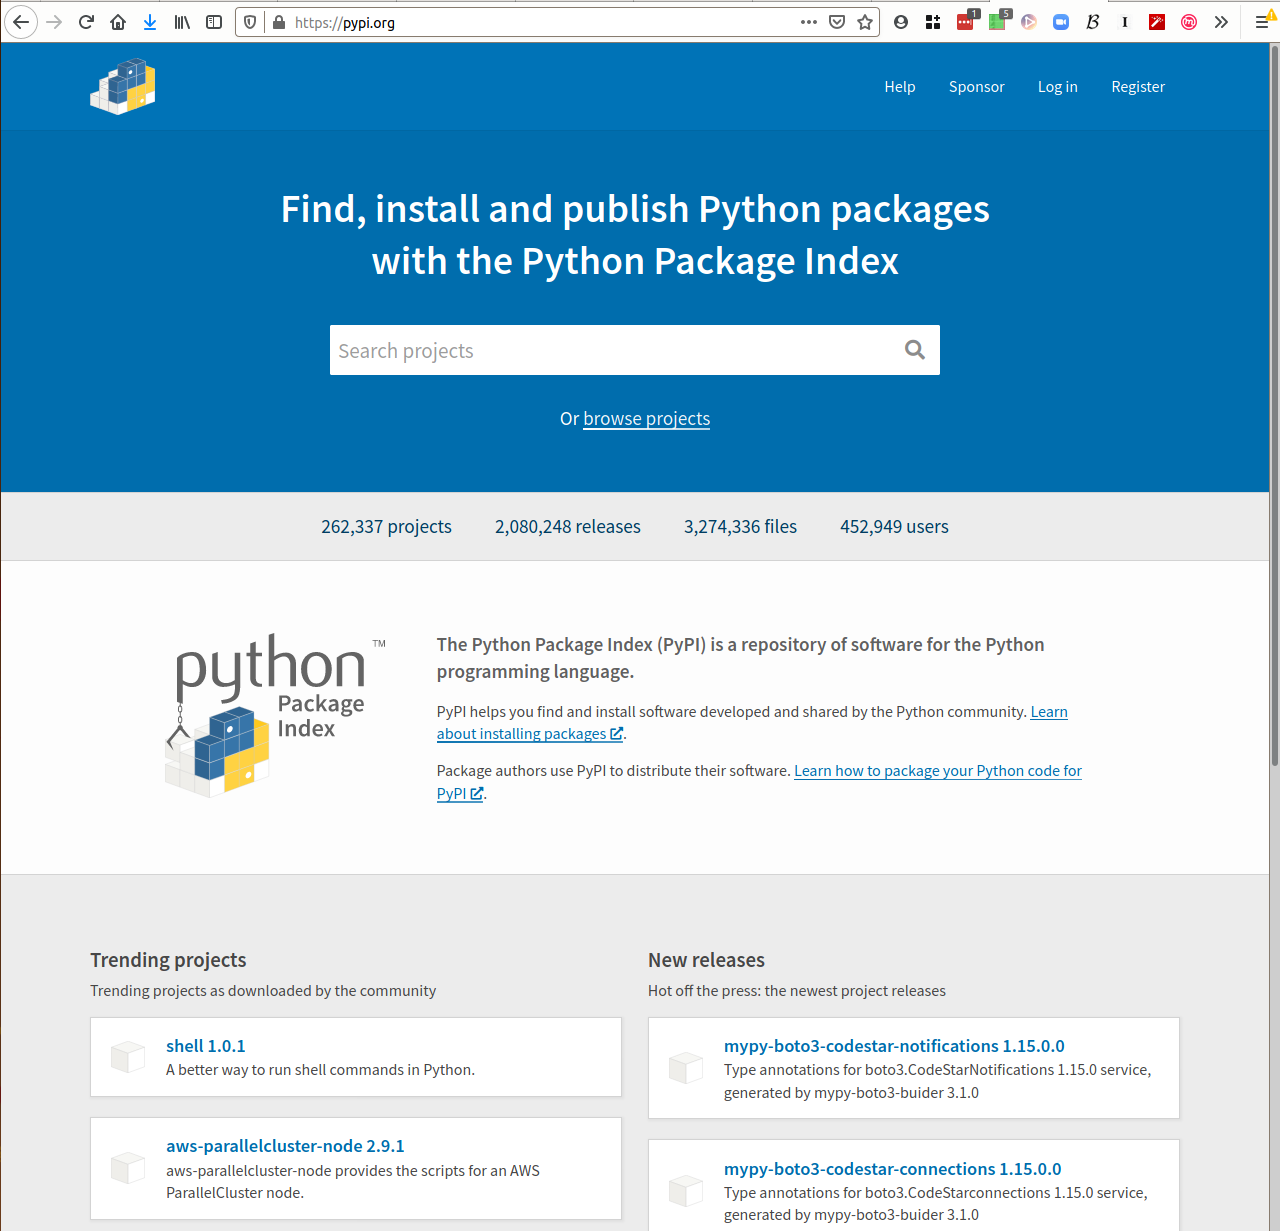
\includegraphics[width=\columnwidth]{figs/pypi.png}
\end{frame}

\begin{frame}
  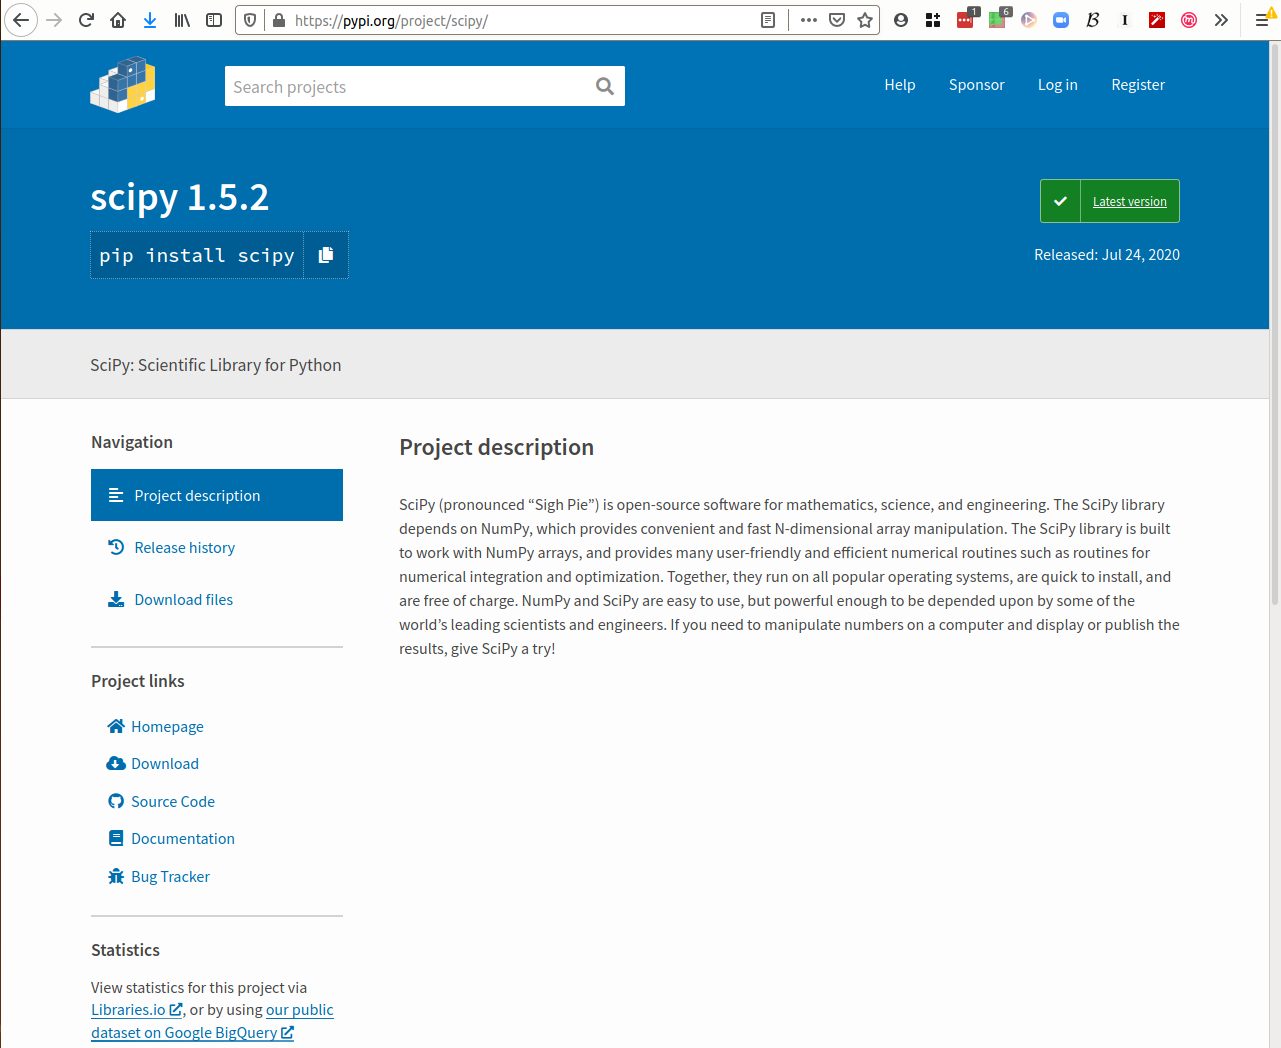
\includegraphics[width=\columnwidth]{figs/pypi-scipy.png}
\end{frame}

\begin{frame}
  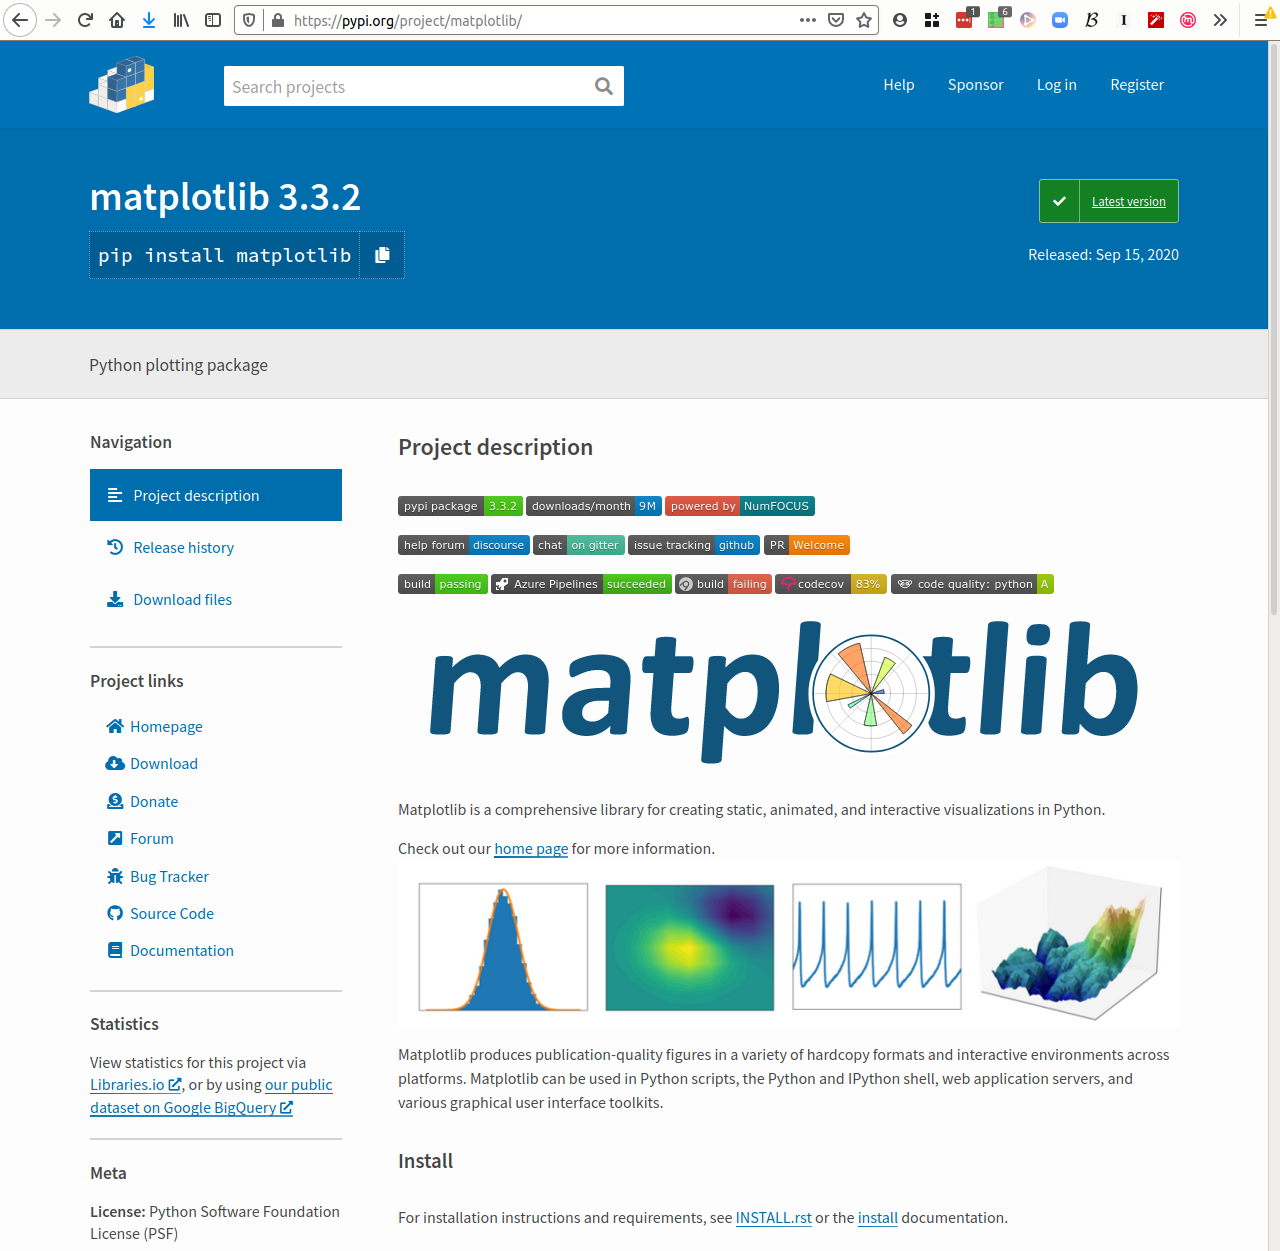
\includegraphics[width=\columnwidth]{figs/pypi-matplotlib.png}
\end{frame}

\begin{frame}[fragile]
  \begin{example}[Installation]
    \begin{minted}{bash}
$ python3 -m pip install numpy scipy matplotlib sympy
    \end{minted}
  \end{example}

  \begin{example}
    \inputminted[lastline=9]{python}{examples/symalg.py}
  \end{example}
\end{frame}

\begin{frame}
  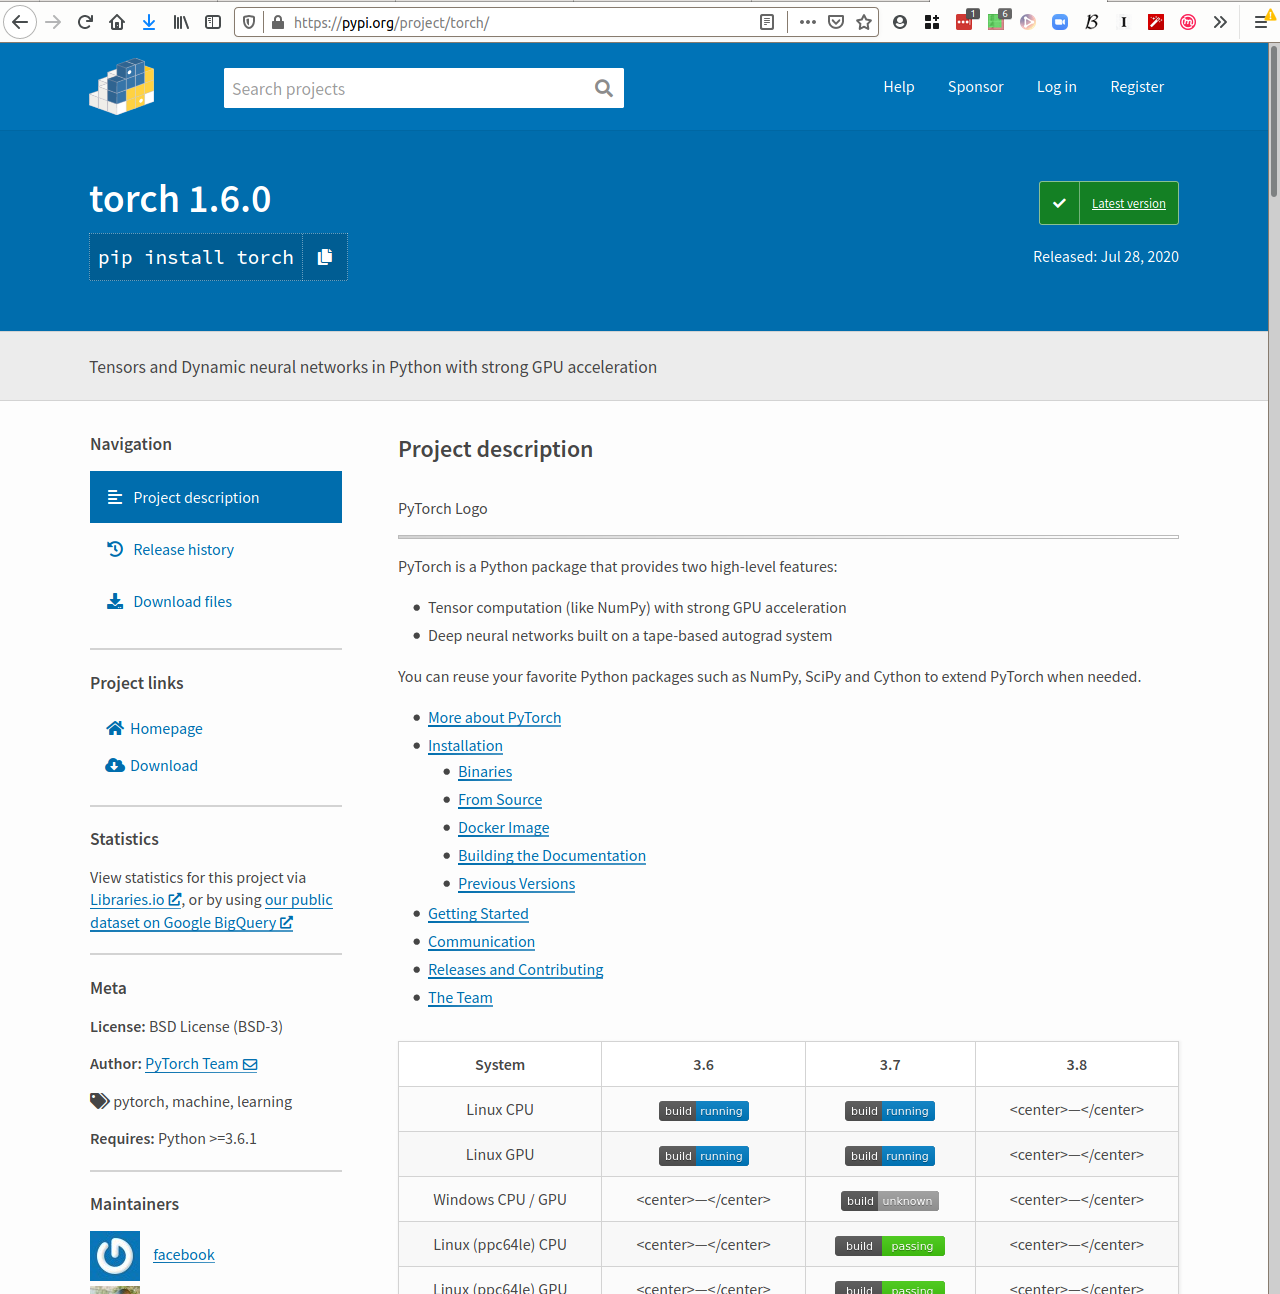
\includegraphics[width=\columnwidth]{figs/pypi-torch.png}
\end{frame}

